\section{Forschungsfragen}

\begin{figure}[htb!]
    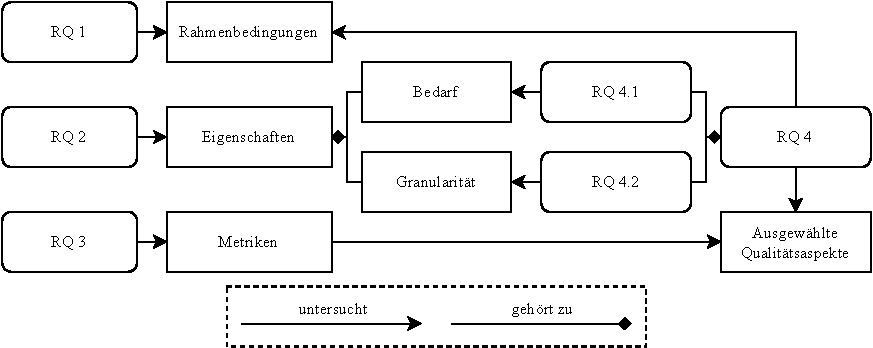
\includegraphics[width=\textwidth]{contents/03_research_design/res/research_questions_overview.pdf}
    \caption{Zusammenhänge der Forschungsfragen}
    \label{fig:research_questions_overview}
\end{figure}

Aus dem Forschungsziel wurden insgesamt fünf Forschungsfragen abgeleitet, welche die Richtung der Arbeit fein granularer definieren. Jede Forschungsfrage behandelt entweder einen konkreten Betrachtungsgegenstand von Erklärbarkeit oder den Zusammenhang der einzelnen Aspekte. Wie die einzelnen Forschungsfragen voneinander abhängen, ist in \autoref{fig:research_questions_overview} dargestellt.

\smallskip

\noindent\fbox{
    \parbox{0.964\textwidth}{
        \smallskip
        \textbf{RQ1} Welche Rahmenbedingungen haben einen Einfluss auf die Anforderungen für Erklärungen?
        \smallskip
    }
}

\smallskip

Erklärbare Systeme können sehr verschiedene Ausprägungen haben (z.B. Empfehlungssystem \cite{kunkel_let_2019} oder Autonome Fahrzeuge \cite{wiegand2019drive}). Auch werden je nach Anwendungsgebiet verschiedene Anforderungen an die Systeme gestellt oder es gibt zusätzlich geltende, äußere Bedingungen \cite{chazette_knowledge_nodate}.

Welche dieser Aspekte einen Einfluss auf die benötigten Erklärungen bzw. Erklärbarkeit im Allgemeinen haben, deckt diese Frage ab. Vor allem konzentriert sich die Frage darauf über welche Rahmenbedingungen sich Stakeholder, die Erklärungen in ein Software-System integrieren möchten, Gedanken machen sollten, um Anforderungen an diese zu formulieren. Dies beinhaltet auch die Ziele, die die Stakeholder für die Software haben.

\smallskip

\noindent\fbox{
    \parbox{0.964\textwidth}{
        \smallskip
        \textbf{RQ2} Welche Eigenschaften von Erklärungen haben einen Einfluss auf die externe Qualität eines erklärbaren Systems?
        \smallskip
    }
}

\smallskip

Es existieren bereits verschiedene Frameworks, welche in bestimmten Kontexten einen Überblick darüber geben, welche Möglichkeiten es gibt, Erklärungen zu gestalten \cite{nunes_systematic_2017}. Vor allem im Bereich der Künstlichen Intelligenz gibt es zahlreiche Arbeiten, welche verschiedene Möglichkeiten vorstellen, um automatisch Erklärungen für komplexe Algorithmen zu generieren \cite{sokol_explainability_2020, mahoney2019framework}.

Um der Forderung nach einem stärkeren Fokus auf den Menschen bei der Betrachtung von Erklärbarkeit nachzukommen \cite{ehsan_operationalizing_2021}, stellt diese Forschungsfrage die externen Qualitätsaspekte \cite{international2011iso} in den Mittelpunkt. Einbezogen werden jene externen Qualitätsaspekte, durch welche die Qualität von Erklärungen bestimmt werden kann. Außerdem werden mit dieser Frage unter anderem die Gestaltungsmöglichkeiten im Rahmen des Bedarfs für Erklärungen und deren Granularität, die Entwicklern oder Designern bei der Konzeption von Erklärungen geboten werden, betrachtet. 

% Folglich ist die Antwort auf diese Frage eine zentrale Grundlage für den Leitfaden, dessen Entwicklung ein Ziel dieser Arbeit ist.

\smallskip

\noindent\fbox{
    \parbox{0.964\textwidth}{
        \smallskip
        \textbf{RQ3} Auf welche Art und Weise kann evaluiert werden, ob die in ein erklärbares System integrierten Erklärungen das Ziel der Integration bezogen auf externe Qualitätsaspekte erfüllt haben?
        \smallskip
    }
}

\smallskip

Erklärbarkeit ist eine NFR, welche von vielen verschiedenen Faktoren abhängt und diese auch beeinflusst \cite{chazette_knowledge_nodate}. Die Integration von Erklärungen hat in der Regel Effekte auf mehrere andere Qualitätsaspekte. Diese können sowohl positiv als auch negativ ausfallen. Ein Problem, welches durch die Integration von Erklärungen leicht entstehen kann, ist, dass sich die \textit{Usability} des Systems verschlechtert, wenn sie nicht explizit mitgedacht wird \cite{sokol_explainability_2020}. Folglich stellt das Messen der Qualität von Erklärungen aufgrund der vielfältigen Effekte eine Herausforderung dar. Ein weiteres Problem bei der Vereinheitlichung ist, dass viele der durch Erklärbarkeit beeinflussten NFRs vor allem subjektiv von Software-Nutzern wahrgenommen werden und somit nur wenige objektive Metriken einsetzbar sind \cite{sokol_explainability_2020}.

In der Literatur wurden bereits Erklärungen anhand verschiedener Metriken analysiert \cite{wiegand2019drive,briand1995goal}. Es fehlt allerdings ein Überblick, welche Metriken zum Messen und zur Bewertung der Qualität von Erklärungen geeignet und erprobt sind. Folglich ist das Ziel bei der Beantwortung dieser offenen Frage, die Metriken, welche bereits zur Evaluation von Erklärungen genutzt wurden, zusammenzutragen.

\smallskip

\noindent\fbox{
    \parbox{0.964\textwidth}{
        \smallskip
        \textbf{RQ4.1} Welchen Einfluss haben die Rahmenbedingungn eines erklärbaren Systems auf den Bedarf für Erklärungen in Bezug auf die externe Qualität des Systems?

        \smallskip

        \textbf{RQ4.2} Welchen Einfluss haben die Rahmenbedingungn eines erklärbaren Systems auf die Granularität von Erklärungen in Bezug auf die externe Qualität des Systems, wenn Erklärungsen notwendig sind?
        \smallskip
    }
}

\smallskip

In den ersten drei Forschungsfragen wurden verschiedene Aspekte von Erklärbarkeit behandelt, die wichtig sind, um darauf basierend Erklärungen in ein System zu integrieren. Es fehlt allerdings die Möglichkeit, anhand der Antworten auf diese Fragen eine Auswahl bei der Gestaltung von Erklärungen zu treffen. Eine Antwort auf diese letzten beiden Fragen soll diesen Prozess unterstützen.

Die Einflüsse, nach denen RQ4.1 fragt, sollen bei der Einschätzung helfen, ob und wenn ja an welchen Stellen, ein System Erklärungen benötigt. Dies soll Entwicklern und Designern dabei helfen, die Frage nach dem Bedarf für Erklärungen Anwendungsfall-übergreifend zu beantworten. Für Navigationsanwendungen haben dies beispielsweise \citeauthor{chazette_end-users_nodate} und \citeauthor{wang_integration_2020} bereits getan \cite{chazette_end-users_nodate,wang_integration_2020}.

Wenn eben dieser Bedarf besteht, muss anschließend die Ausgestaltung dieser Erklärung betrachtet werden. Welche bereits untersuchten Einflüsse in Bezug auf diese Granularität von Erklärungen bestehen, soll die Antwort auf die Frage RQ4.2 beantworten.

Folglich stellen die Forschungsfragen RQ4.1 und RQ4.2 die Schnittstelle zwischen den ersten drei Forschungsfragen dar.

% \bigskip

% Die Vorgehensweise dieser Arbeit zum Erreichen des vorgestellten Ziels und bei der Beantwortung der aus dem Ziel abgeleiteten Forschungsfragen wird im folgenden Abschnitt vorgestellt.